\section{Câu hỏi 2: Các đợt lưu lượng cao}

Q95 toàn chuỗi là \QHigh{} m³/s. Có \NDaysHigh{} ngày vượt ngưỡng, chiếm \ShareHigh\%
chuỗi, gom thành \NEvents{} đợt liên tiếp. Đợt dài nhất kéo dài \LongestEvent{} ngày;
đỉnh lớn nhất trong các đợt là \MaxEventPeak{} m³/s, thuộc năm 2017. Việc gộp các ngày
liên tiếp giúp phân biệt một đợt kéo dài với nhiều dao động ngắn.

\begin{figure}[H]
\centering
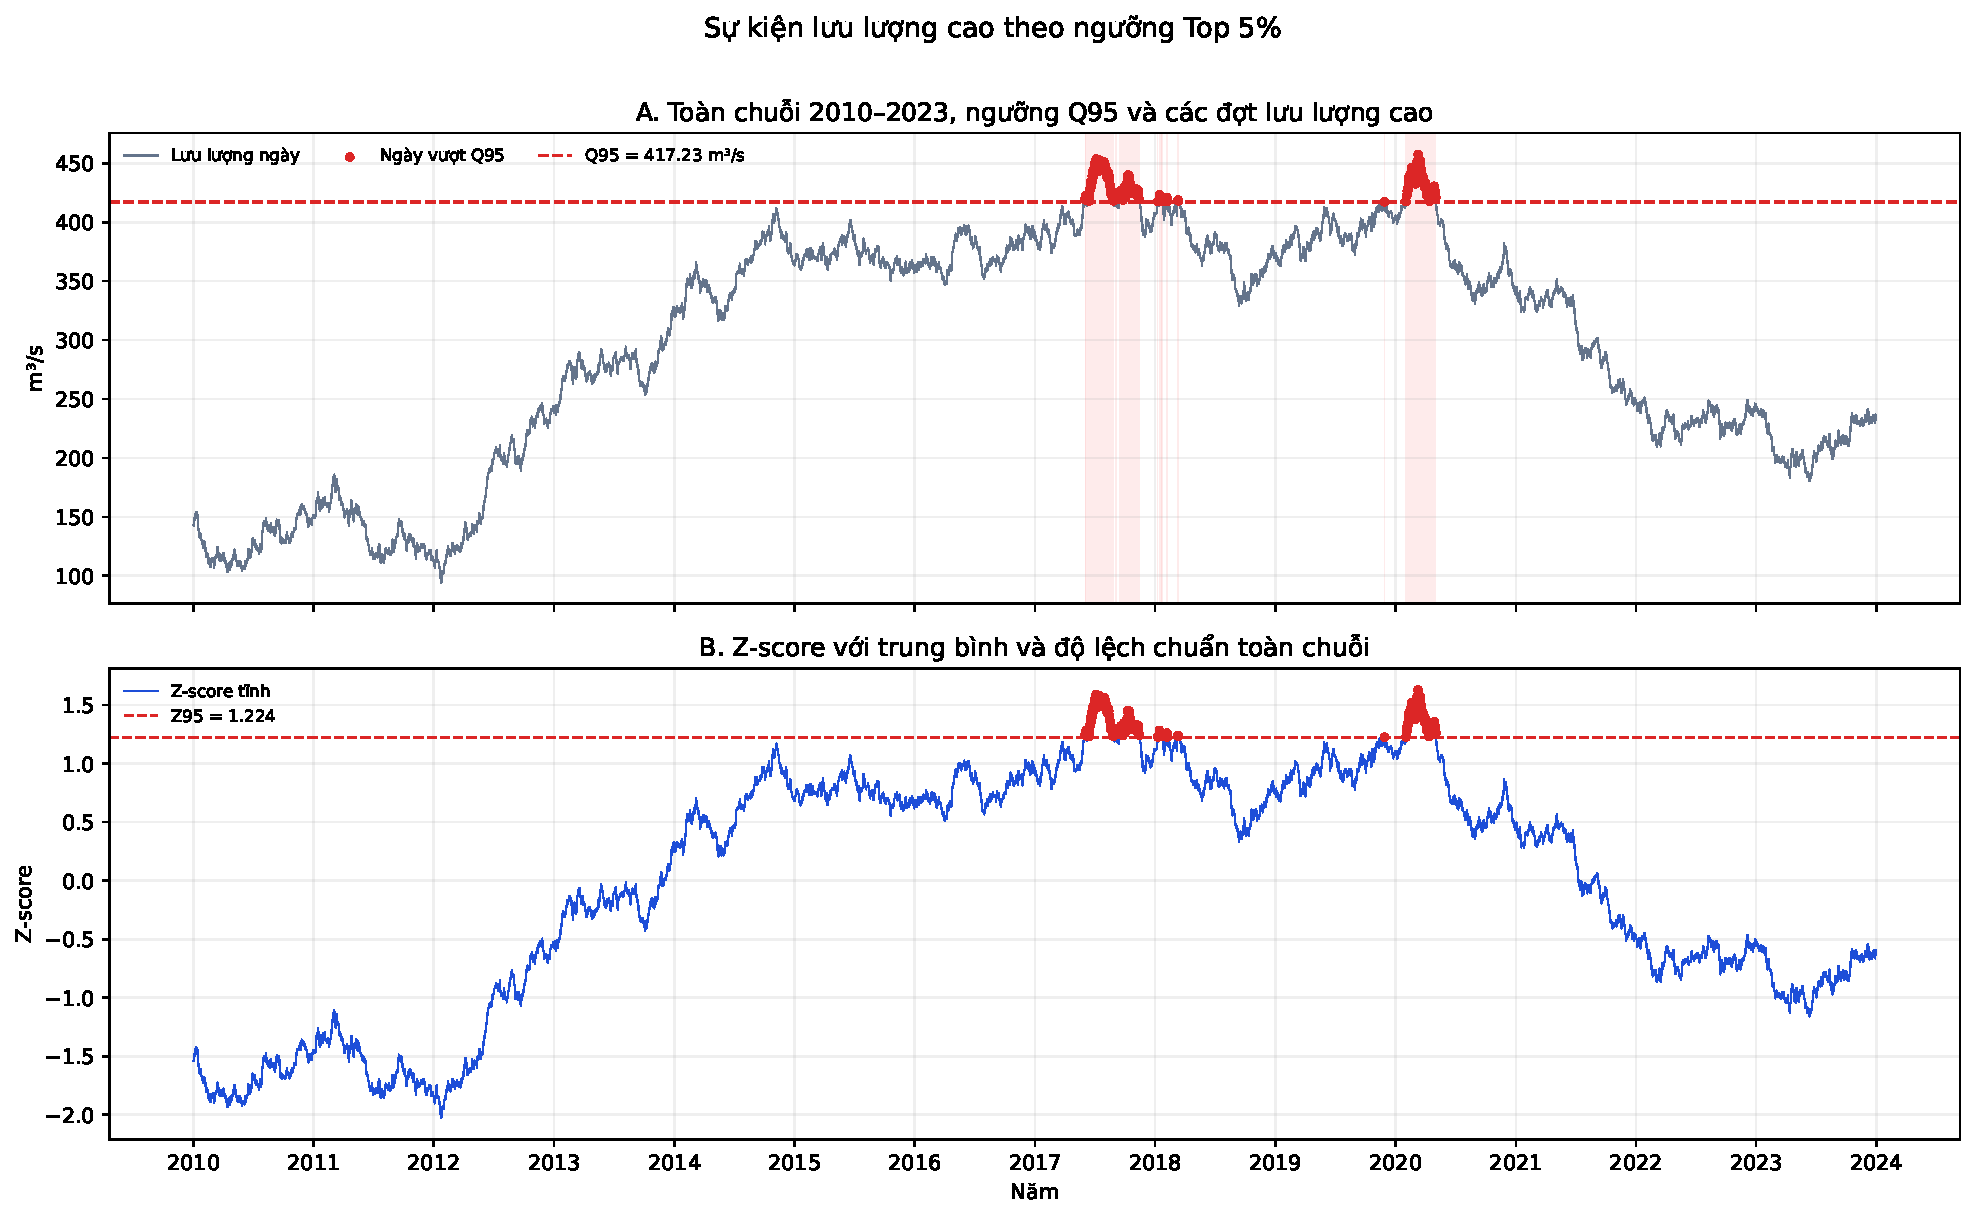
\includegraphics[width=0.86\linewidth]{figures/extremes_full_series.pdf}
\caption{Chuỗi lưu lượng và các ngày vượt Q95. Các đợt tập trung chủ yếu quanh
2017--2020.}
\label{fig:q2}
\end{figure}

\begin{table}[H]
\centering
\caption{Top 5 đợt theo đỉnh lưu lượng}
\label{tab:top5}
\small
\begin{tabular}{clrrr}
\toprule
Hạng & Khoảng ngày & Số ngày & Ngày đỉnh & Đỉnh (m³/s) \\
\midrule
1 & 04/02/2020–03/05/2020 & 90 & 10/03/2020 & 457{,}49 \\
2 & 13/06/2017–28/08/2017 & 77 & 06/07/2017 & 453{,}52 \\
3 & 15/09/2017–14/11/2017 & 61 & 11/10/2017 & 439{,}97 \\
4 & 02/09/2017–05/09/2017 & 4 & 03/09/2017 & 423{,}71 \\
5 & 13/01/2018–16/01/2018 & 4 & 14/01/2018 & 423{,}21 \\
\bottomrule
\end{tabular}

\end{table}

Bảng~\ref{tab:top5} cho thấy đợt dài nhất (90 ngày, đầu năm 2020) không phải đợt có
đỉnh lớn nhất; đỉnh lớn nhất nằm trong đợt tháng 6--8/2017. Vì ngưỡng Q95 tính trên
toàn chuỗi, số ngày vượt ngưỡng trong một năm cụ thể có thể cao hơn hoặc thấp hơn 5\%.
Kết quả này chỉ mô tả các đợt trong dữ liệu, không phải phân vùng rủi ro lũ.
